\documentclass[11pt,a4paper]{article}
\author{TalentSprint}
\date{}
\usepackage{verbatim}
\usepackage{fancyhdr}           % For header and footer
\usepackage{multicol}
\usepackage{colortbl}           % For coloured tables
\usepackage{setspace}           % For line height
\usepackage{seqsplit}           % Splits long words.
\usepackage{amsmath} 
\usepackage{graphicx}
\usepackage{array}
\usepackage{enumitem}
\usepackage{xcolor}
\usepackage[tikz]{bclogo}
\usepackage{textcomp}
\usepackage{listings}
\lstset{language=python,numbers=left,numberstyle=\tiny,numbersep=10pt,showstringspaces=false}

\headheight=14pt
\lhead{\nouppercase{}}
\rhead{\nouppercase{\leftmark}}

\graphicspath{{../Images/} {../ScreenShots/}}
\setcounter{tocdepth}{1}
\setlength\parindent{0pt}
\parskip=4pt
\newcommand{\Code}[1]{\textbf{\texttt{#1}}}

\begin{comment}
\def\AnswerBox{\fbox{\begin{minipage}{4in}\hfill\vspace{0.5in}\end{minipage}}}

\thispagestyle{empty}
\vspace{1.5pc}
\topskip0pt
\vspace*{\fill}
\centerline{\Huge Modern Programming}
\vspace{2pc}
\centerline{\Huge Practice}
\vspace{2pc}
\centerline{\Large using Python}
\vspace*{\fill}
\centerline{Prepared by TalentSprint WISE Team} 
\setcounter{page}{1}


\end{comment}
%========================================================================

% Lengths and widths
\addtolength{\textwidth}{5cm}
\addtolength{\hoffset}{-1cm}
\setlength{\headsep}{-12pt} % Reduce space between header and content
\setlength{\headheight}{85pt} % If less, LaTeX automatically increases it
\renewcommand{\footrulewidth}{2pt} % Remove footer line
\renewcommand{\headrulewidth}{1pt} % Remove header line
\renewcommand{\seqinsert}{\ifmmode\allowbreak\else\-\fi} % Hyphens in seqsplit
% This two commands together give roughly
% the right line height in the tables
\renewcommand{\arraystretch}{1.3}
\onehalfspacing



% Commands
\newcommand{\SetRowColor}[1]{\noalign{\gdef\RowColorName{#1}}\rowcolor{\RowColorName}} % Shortcut for row colour
\newcommand{\mymulticolumn}[3]{\multicolumn{#1}{>{\columncolor{white}}#2}{#3}} % For coloured multi-cols
\newcolumntype{x}[1]{>{\raggedright}p{#1}} % New column types for ragged-right paragraph columns
\newcommand{\tn}{\tabularnewline} % Required as custom column type in use

% Font and Colours
\definecolor{HeadBackground}{HTML}{333333}
\definecolor{FootBackground}{HTML}{666666}
\definecolor{TextColor}{HTML}{333333}
\definecolor{DarkBackground}{HTML}{6B8E23} %{FD1AA8}
\definecolor{LightBackground}{HTML}{E8FED8} %D3FDC8
\definecolor{tit}{HTML}{FF6600}
\renewcommand{\familydefault}{\sfdefault}
\color{TextColor}
 \headsep = 25pt
% Header and Footer
\pagestyle{fancy}
\usepackage[headheight=110pt]{geometry}
\fancyhf{}% Clear header/footer

\fancyhead[r]{
\includegraphics[width = 4cm, height = 2cm]{TS-Logo.png}\hspace{0cm}}

%=================================TITLE=====================================
\fancyhead[l]{\Large{\bf{\textcolor{tit}{\textrm{Conditional statements}}}}}
%===========================================================================

\renewcommand{\headrulewidth}{0.4pt}% Default \headrulewidth is 0.4pt
\renewcommand{\footrulewidth}{0.4pt}% Default \footrulewidth is 0pt

\rfoot{Page \thepage}
\lfoot{COPYRIGHT \textcopyright TALENTSPRINT, 2015. ALL RIGHTS RESERVED.}




\begin{document}



%\chapter*{Conditional statements}

We need to execute different sections of code under different circumstanes. For example, in a billing situation a credit card may attract additional charges or a bill amount higher than a fixed amount may get discount.  In order to check different conditions and execute different code we need conditional execution. This is almost always achieved using \Code{if} in all programming languages. Python is no different.

\section*{Booleans:  Overview}
A boolean expression is an expression that is either true or false. One way to write the boolean expression is to use the operator ==, which compares two values and produces a boolean value:
\begin{verbatim}
>>> 6 == 6
True
>>> 5 == 6
False
\end{verbatim}
In the first statement,the two operands are equal, so the value of the expression is True, in the second statement, 5 is not equal to 6, so we get False. True and False are special values that are built into Python.

The == operator is one of the comparision operators; the others are:

\begin{table}[ht]
\centering
\begin{tabular}{|c|c|}\hline
\textbf{Expression}    &    \textbf{Description}\\\hline
x ! = y     &      x is not equal to y\\\hline
x $>$ y        &     x is greater than y\\\hline
x $<$ y        &     x is less than y\\\hline
x $>=$ y      &    x is greater than or equal to y\\\hline
x $<=$ y      &    x is less than or equal to y\\\hline
\end{tabular}
\end{table}
Although these operations are probably familiar to you, the Python symbols are different from the mathematical symbols.
A common error is to use a single equal sign(=) instead of a double equal sign(==). Remember that = is an assignment operator and  == is a comparision operator.

\section*{Simple if statement}
The simplest form of \Code{if} statement is one where a piece of code is executed if a condition exists otherwise nothing is done. For example:
\begin{verbatim}
if x > 0:
    print("x is positive")
\end{verbatim}
The boolean expression after the \Code{if} statement is called the condition. If it is true, then the indented statement gets executed, If not, nothing happens.

\begin{description}
\item[Example ] Program to check whether the number is even or odd.
\begin{lstlisting}
n = 10
if n % 2 == 0:
    print(n, "is Even")
if n % 2 != 0:
    print(n, "is Odd")
\end{lstlisting}

\begin{figure}[ht]
\begin{center}
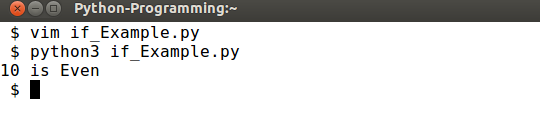
\includegraphics[scale=0.4]{Output_ifExample.png}
\caption{If Example}
\label{If_Example}\end{center}
\end{figure}
\end{description}

\section*{Blocks in Python}
Like other compound statements, the \Code{if} statement is made up of a header and a block of statements:
\begin{verbatim}
HEADER:
    FIRST STATEMENT
    ...........
    ...........
    LAST STATEMENT
\end{verbatim}
The header begins on a new line and end with a colon(:). the indented statements that follow are called \Code{block}. The first unindented statement marks the end of the block. A statement block inside a compound statement is called the \Code{body} of the statement.

\section*{if \ldots else}
This is another form of \Code{if} statement, in which there are two possibilities and the condition determines which one gets executed. Contrast this to the simple if, where if the condition is not true nothing is done.
We look at the program to understand how if \ldots else works:
\begin{verbatim}
if x % 2 == 0:
    print(x, "is Even")
else:
    print(x, "is Odd")
\end{verbatim}
If the remainder of the condition is ``Zero'', then we know that \Code{x} is Even, and the program displays a message. If the condition is false, the second set of statements is executed. Since the condition must be \Code{true} or \Code{false}, exactly one of the alternative will be executed. The alternatives are called \Code{branches}, because they are branches in the flow of execution.

\begin{description}
\item[Example ] Accept marks and check whether the student is passed or failed in a test. 
\begin{lstlisting}
marks = 76
if marks >= 45:
    print("Passed")
    print("Congratulations!!")
else:
    print("Failed")
    print("Good luck in the retest")
\end{lstlisting}

\begin{figure}[ht]
\begin{center}
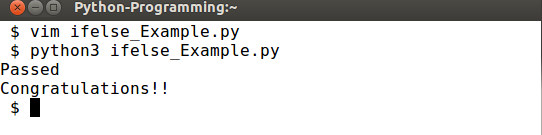
\includegraphics[scale=0.4]{Output_ifelse_Example.png}
\caption{If Example}
\label{If_Example}\end{center}
\end{figure}
\end{description}

\section*{Nested if}
One if statement within an another if, such as conditional statement inside a branch of another conditional statement is termed as nested if.
We look at the program to understand how nested if works:
\begin{verbatim}
# Check whether the number is even or odd if it is positive.
x = 56
if x >= 0:  # Outer if 
    if x % 2 == 0:  # Inner if
        print(x, "is Even Number")
    else:
        print(x, "is Odd Number")
else:
    print(x, "is Negative")
\end{verbatim}
The outer condition is evaluated first, as the condition is true it gets into the block and evaluates an inner condition and it prints ``\Code{x} is Even Number'' as the condition is true. If it fails it executes the else block of statement and prints ``\Code{x} is an Odd Number''. If the outer condition itself evaluates to false then it executes the else part of it and it prints ``\Code{x} The Number is Negative''.
\section*{Compound Conditions}\
Compound conditions are formed by combining multiple conditions in a statement. We use logical operators to form compound conditions.
\begin{description}
\item[Example 01] Given three sides of a triangle find out, if it is equilateral.
\begin{verbatim}
if a == b and b == c:
    print("Equilateral triangle")
else:
    print("Not an equilateral triangle")
\end{verbatim}
We used logical operator \Code{and} in the above example to combine two conditions.
If the value of three variables \Code{a}, \Code{b} and \Code{c} are equal then the condition evaluates to true and prints ``Equilateral Triangle''.

\item[Example 02] Given three angles of a triangle and check whether it is right-angled triangle.
\begin{verbatim}
if x == 90 or y == 90 or z == 90:
    print("Right Angled Triangle")
else:
    print("Not a Right Angled Triangle")
\end{verbatim}
We use logical operator \Code{or} in the above example to combine multiple conditions.
If any of the value is equal to 90 then the condition evaluates to true and prints ``Right Angled Triangle''.
\end{description}
As we know that logical operators often provide a way to simplify nested conditional statements. For Example, we can rewrite the following code using a single condition:
\begin{lstlisting}
if 0 < x:
    if x < 10:
        print "x is a positive single digit."
\end{lstlisting}
The \Code{print()} statement is executed only if we make it past both the conditionals, so we can use the \Code{and} operator:
\begin{lstlisting}
if 0 < x and x < 10:
    print "x is a positive single digit."
\end{lstlisting}
These type of conditions are commonly used, so Python provides an alternative syntax that is similar to mathematical notation:
\begin{lstlisting}
if 0 < x < 10:
    print "x is a positive single digit."
\end{lstlisting}
This condition is semantically the same as the compound condition and the nested condition.

\section*{if \ldots elif \ldots else}
Sometimes there are more than two possibilities and we need more than two branches. One way to express a computation like that is a series of conditions. In such cases we use \Code{if \ldots elif \ldots else}.

\Code{elif} is an abbreviation of ``else if''. The conditions are checked one after another. The statement associated with the first true condition is executed. There is no limit of the number of \Code{elif} statements, but the last branch has to be an else statement:
\begin{verbatim}
if x < y:  # Condition 1
    print(x, "is less than", y)
elif x > y:  # Condition 2
    print(x, "is greater than", y)
else:
    print(x, "and", y, "are equal")
\end{verbatim}
In the above example, Condition 1 is evaluated first, if it is true it executes the associated block of statements. If it fails Condition 2 is evaluated and if it is true it executes the associated block of statements otherwise it executes the else block of statements.

\begin{description}
\item[Example ] Find the grade of a student based on a marks.
\begin{lstlisting}
marks = 75
if marks >= 80:
    print("Grade A")
elif marks >= 60:
    print("Grade B")
elif marks >= 40:
    print("Grade C")
else:
    print("Failed")
\end{lstlisting}
\begin{figure}[ht]
\begin{center}
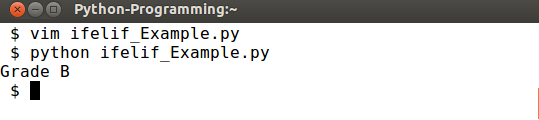
\includegraphics[scale=0.4]{Output_ifelif_Example.png}
\caption{Ifelif Example}
\label{Ifelif_Example}\end{center}
\end{figure}
\end{description}

\end{document}